\documentclass[12pt,letterpaper]{report}
\usepackage[margin=1in,includeheadfoot]{geometry}
\usepackage[hidelinks,bookmarksnumbered]{hyperref}
\usepackage[figure,table]{hypcap}
\usepackage[nottoc]{tocbibind}
\usepackage[titletoc]{appendix}
\usepackage[utf8]{inputenc}
\usepackage[T1]{fontenc}
\usepackage{todonotes}

\usepackage{fancyhdr}
\pagestyle{fancy}
\fancyhf{}
\rhead{\textit{\leftmark}}
\cfoot{\thepage}
\renewcommand{\headrulewidth}{0pt}

\usepackage[backend=biber,sorting=none]{biblatex}
\addbibresource{references.bib}

\usepackage{graphicx}
\graphicspath{ {images/} }

\usepackage{setspace}
\onehalfspacing

\usepackage{datetime}
\newdateformat{monthyeardate}{\monthname[\THEMONTH] \THEYEAR}
\newdateformat{yeardate}{\THEYEAR}

\usepackage{sectsty}
\chapterfont{\vspace*{-14.88mm}\large\sc\centering}
\chaptertitlefont{\centering}
\subsubsectionfont{\centering}

%----------------
% Title Page
%----------------
\begin{document}

\begin{titlepage}
	\begin{center}
		\vspace*{1in}
		
		\Huge
		Thesis Title
		
		\vfill
		
		\large
		Cheuk Chuen Siow\\
		School of Computer Science\\
		McGill University, Montréal
		
		\vfill
		
		\monthyeardate\today
		
		\vfill
		
		A thesis submitted to McGill University in partial fulfillment of the requirements for the degree of Master of Science in Computer Science
		
		\vfill
		
		\textcopyright{} Cheuk Chuen Siow \yeardate\today
		
		\vspace*{1in}
	\end{center}
\end{titlepage}

%----------------
% Front Matter
%----------------
\clearpage
\pagenumbering{roman}
\setcounter{page}{2}

\chapter*{Abstract}
\addcontentsline{toc}{chapter}{Abstract}



\clearpage

\chapter*{Abrégé}
\addcontentsline{toc}{chapter}{Abrégé}



\clearpage

\chapter*{Acknowledgements}
\addcontentsline{toc}{chapter}{Acknowledgements}



\clearpage

\chapter*{Preface}
\addcontentsline{toc}{chapter}{Preface}



% Content
\renewcommand{\contentsname}{Table of Contents}
\tableofcontents
\listoffigures
\listoftables

\clearpage
\pagenumbering{arabic}

%----------------
% Main Body
%----------------
\chapter{Introduction}
% !TEX root = ../thesis.tex

Since 1960s, software development has been evolving rapidly to address the increasing demands of complex software. The complexity of modern software brings about difficulties in developing and maintaining quality software. Software engineering as a discipline ensures that developers follow a systematic production of software, by applying best practices to maximize quality of deliverables and minimize time-to-market. Various methodologies exist through the efforts of active research by theorists and practitioners, but the core of software development process typically consists of the following six phases---requirements gathering, design, implementation, testing, deployment, and maintenance.

Conceptual models help illustrates complex systems with a simple framework by creating abstractions to alleviate the amount of complexity. Hence, the use of models is progressively recommended in representing a software system. This simplifies the process of design, maximizes compatibility between different platforms, and promotes communication among stakeholders. Model-Driven Engineering (MDE) technologies offer the means to represent domain-specific knowledge within models, allowing modelers to express domain concepts effectively~\cite{schmidt2006model}. MDE advocates using the best modeling formalism that expresses relevant design intent declaratively at each level of abstraction. During development, we can use models to describe different aspects of the system vertically, in which the models are refined from higher to lower levels of abstraction through model transformation. At the lowest level, models use implementation technology concepts, and appropriate tools can be used to generate code from these platform-specific models~\cite{sendall2003model}.

Modularity is key in designing computer programs that are extensible and easily maintainable, but concerns that are crosscutting and more scattered in the implementation are more likely to cause defects~\cite{eaddy2008crosscutting}. This poses obstacles for MDE because modeling such crosscutting concerns in a modular way is difficult from an object-oriented standpoint. Furthermore, reusability is also a main factor in allowing developers to leverage reusable solutions such as libraries and frameworks provided for a given programming language, thereby improving the development speed without having to implement existing software components from first principles. Model reuse is still in its early stage, but modeling libraries are emerging as well~\cite{france2012repository}.

Concern-Oriented Reuse (CORE) is a new software development paradigm or approach that puts reuse at the forefront of software development~\cite{alam2013concern}. In CORE, software development is structured around modules called \emph{concerns} that provide a variety of reusable solutions for recurring software development issues. Techniques from MDE, Software Product Lines (SPL) engineering, and software composition (in particular feature-orientation and aspect-orientation) allow concerns to form modular units of reuse that encapsulate a set of software development artifacts, i.e., models and code, during software development in a versatile, generic way.

The main premise of CORE is that recurring development concerns are made available in a concern library, which eventually should cover most recurring software development needs. Similar to class libraries in modern programming languages, this library should grow as new development concerns emerge, and existing concerns should continuously evolve as alternative architectural, algorithmic, and technological solutions become available. Applications are built by reusing existing concerns from the library whenever possible, following a well-defined reuse process supported by clear interfaces. To generate an executable in which concerns exhibit intricate crosscutting structure and behavior, CORE relies on additive software composition techniques, feature-oriented technology, and aspect-oriented technology.

Currently, CORE only supports modelling notations that are used at the design phase~\cite{kienzle2010aspect}. In order to fully integrate CORE with MDE, other development phases should also be supported. We are interested in adding support for requirements modeling languages to CORE, so that requirements modellers too can benefit from advanced modularization and reuse support. We chose to concentrate on the User Requirements Notation (URN), which sets the standard as a visual notation for modeling and analyzing requirements~\cite{amyot2002urn}. URN formalizes and integrates two complementary languages: (i) Goal-oriented Requirements Language (GRL) to describe non-functional requirements as intentional elements, and (ii) Use Case Map (UCM) to describe functional requirements as causal scenarios. GRL and UCM are used to capture goal and scenario models, respectively. Since CORE already supports the use of goal models to analyze the impact of choosing features~\cite{alam2013concern}, this thesis focuses on integrating scenario models with the concepts of CORE.

\section{Contributions}

This thesis advances the state-of-the-art in modeling by proposing a complete solution for augmenting the UCM modeling notation with CORE capabilities, resulting in a variant of UCM---Concern-Oriented Use Case Maps (CoUCM). Specifically, the thesis makes the following contributions:

\begin{itemize}

\item A metamodel for CoUCM that extends the CORE metamodel, thus formalizing the integration of the CORE concepts into the UCM language.

\item A CORE-compatible weaving algorithm for CoUCMs that takes as an input two CoUCM models and produces a composed CoUCM model. This makes it possible for requirements engineers to modularize scenarios according to concern features (i.e., a weaving algorithm compatible with CORE extension) as well as to reuse existing scenarios when creating new ones (i.e., compatible with the CORE reuse mechanism).

\item An implementation of the proposed CoUCM metamodel and weaving algorithm in TouchCORE, serving as a proof of concept validation.

\item A demonstration of the expressiveness and reuse potential of CoUCMs by means of an \emph{Authentication} concern and an \emph{Online Payment} concern, and two \emph{Workflow Patterns} case studies.

\end{itemize}

\section{Thesis Outline}

The remainder of this thesis is structured as follows. Chapter~\ref{ch:2} offers background information on CORE and UCM, as well as presents existing modeling techniques closely related to our work. Chapter~\ref{ch:3} details the integration of CORE with UCM, namely the CoUCM meta model and the different CoUCM weaving algorithms. Chapter~\ref{ch:4} validates the proposed meta model
and weaving algorithms by presenting some details of the TouchCORE implementation. Finally, Chapter~\ref{ch:5} concludes the thesis and discusses possible future work.


\chapter{Background} \label{ch:2}
First paragraph opens with URN and its components.

\section{Use Case Map (UCM)}

This section describes UCM in detail.

\section{Concern-oriented Reuse (CORE)}

This section describes CORE in detail.

\subsection{Reusable Aspect Models (RAM)}

\section{Overview of Relevant Modeling Tools}

Literature review.

\section{Motivation}

Build on the motivation of having UCM as an additional model for TouchCORE.

\subsection{UCM in the Context of CORE}

Weaving, extending, and reusing UCM concern models.

Last paragraph leads to implementation chapter.


\chapter{Adding Support for UCM to CORE} \label{ch:3}
\todo[inline]{How about as a title: Adding Support for Use Case Maps to CORE}

\todo[inline]{Then talk about (or remind the reader about) motivation, then detail that there needs to be support in the metamodel, the concrete syntax, and the weaving algorithm. It could also be possible to not talk about the concrete syntax here, but in the next chapter (the implementation). This chapter really describes the conceptual work of adding UCMS to CORE.}

\section{UCM Metamodel}

\subsection{Abstract Syntax}

\subsection{Concrete Syntax}

\todo[inline]{Maybe move this to the next chapter... To discuss}

\section{Weaver}

\todo[inline]{Again, maybe we need a short intro here. I assume there is also a common algorithm to extensions and reuses, or are they completely separate?}

\subsection{Model Extension}

\subsection{Model Reuse}


\chapter{Validation} \label{ch:4}
The definition of UCM metamodel and the specification of weaving algorithm described in the previous chapter provide the foundation for the implementation of UCM in TouchCORE, a multitouch-enabled concern-oriented software design modeling tool. In this chapter, we illustrate the realization of scenario models in TouchCORE through the use of UCM notation in section~\ref{sec:4.1}. Then we attempt to validate our proposed approach of concern-oriented UCMs by means of case studies in section~\ref{sec:4.2}. Finally, we demonstrate that concern-oriented UCMs are able to cover the workflow patterns in section~\ref{sec:4.3}.

\section{UCM Implementation in TouchCORE} \label{sec:4.1}

TouchCORE is under active development within the Software Engineering Lab at McGill University \cite{sel2015touchcore}. Previous project, TouchRAM, successfully implemented concern-oriented software design paradigm, but support is limited to RAM (class, sequence, and state diagrams) \cite{al2012touchram, schottle2014touchram}. TouchCORE extends TouchRAM with numerous enhancements, most notably the support for arbitrary modeling languages in addition to RAM. Since we have a well-defined corified UCM metamodel, we attempted to add support for UCMs in TouchCORE as proof of concept, enabling TouchCORE the capability to build scalable and reusable scenario models.

The project uses Java SE Development Kit 8 as the implementation language and Eclipse Modeling Framework (EMF)~\cite{steinberg2008emf} as the modeling facility for developing TouchCORE. To support a new language, we need to define its metamodel based on Ecore. TouchCORE already has a complete CORE metamodel defined with an Ecore model (see Figure~\ref{fig:a.1}). With RAM as a reference model, we constructed an Ecore model that expresses our complete UCM metamodel, subclassing the appropriate CORE metaclasses, through the use of EMF tooling (see Figure~\ref{fig:a.2} in Appendix~\ref{ch:A} for complete UCM metamodel). EMF is capable of generating structured Java code from valid Ecore models, allowing us to rapidly program the logic for UCM integration.

\begin{figure}
	\centering
	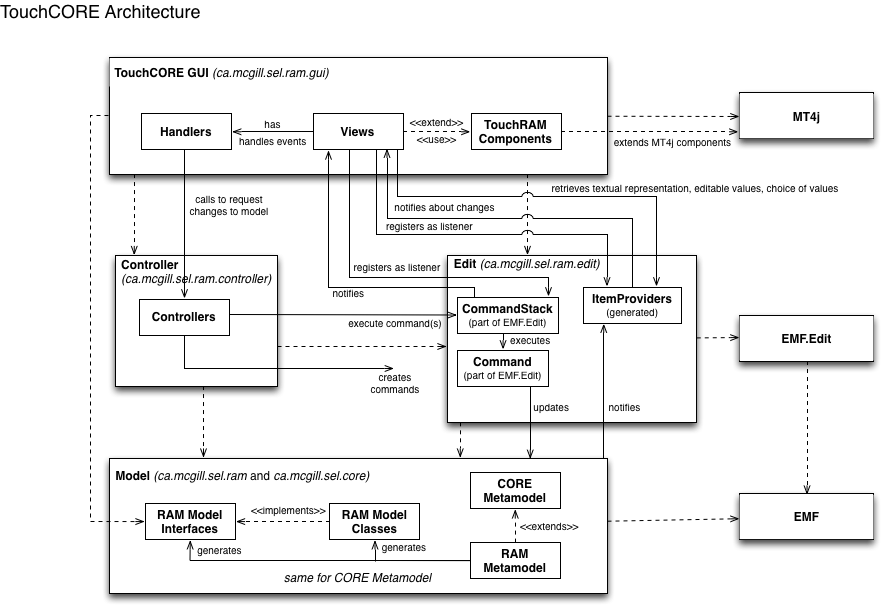
\includegraphics[scale=0.5]{fig_4_1.png}
	\caption[TouchCORE architecture]{TouchCORE architecture. Image courtesy of Software Engineering Lab, McGill University}
	\label{fig:4.1}
\end{figure}

The software architecture of TouchCORE follows the model–view–controller (MVC) design pattern to separate the program into three main logical components. Figure~\ref{fig:4.1} shows the three interconnected parts for the TouchCORE application: (i) the model layer for managing data, e.g., instances of RAM and UCM models; (ii) the TouchCORE graphical user interface (GUI) that constitutes the view layer for visualizing and manipulating models; and (iii) the controller layer for handling user interactions and act on the data model objects. The GUI for TouchCORE is built on top of MT4j for its multitouch capability \cite{laufs2010mt4j}. Additional components include weaver, code generator, model validator, and classloader. The integration of UCM in TouchCORE involves modifying its core components with varying degrees, but the program is structured in such a way that we can add subcomponents when implementing a new modeling language, adhering to the open/closed principle.

\subsection{Supported Concrete Syntax}

\begin{figure}[h]
	\centering
	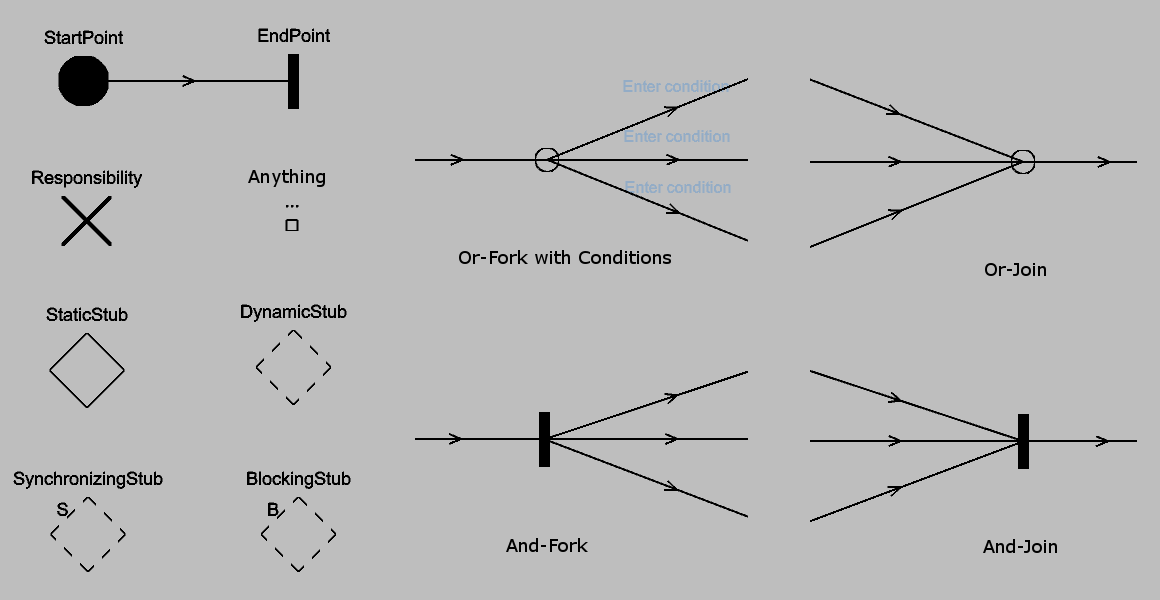
\includegraphics[scale=0.3]{fig_4_2.png}
	\caption{UCM notation in TouchCORE}
	\label{fig:4.2}
\end{figure}

The basic elements of the UCM notation that we implemented in TouchCORE are shown in Figure~\ref{fig:4.2}. Most of these elements are defined by the standards~\cite{itu2012151}, with the exception of {\cls Anything} that is taken from the extended AoUCM metamodel~\cite{mussbacher2011aspect}. Users can create path nodes by tap-and-hold on the canvas of TouchCORE during runtime and a list of path nodes will be displayed for selection. To create a node connection between two path nodes, simply drag from the area adjacent of one element to the other element.

There are several anomalies with regards to the graphical representation of UCM symbols displayed in TouchCORE as compared with the standards (compare Figure~\ref{fig:4.2} with Figure~\ref{fig:2.7}). For example, the symbol for OR-fork and OR-join is shown as a circle instead of no symbol (just direct branching and merging from the paths); anything is represented as a square with the label \ldots\ instead of just \ldots; and node connection is a straight line path instead of spline. These are some of the limitations that we faced at the moment when implementing the GUI. Our current method of creating nodes is to first create them on the canvas, then build the connections later. OR-fork and OR-join need a space to receive events from the user, thus a circle serves as the area of interactivity as well as a statement of presence that an OR-fork or OR-join has been created. The idea of displaying the \ldots symbol of an anything node is that it should be part of the node connection and move along seamlessly with correct orientation whenever the predecessor or successor node of anything is moved, but since anything is considered a path node, we decided for now to just use a square with the label \ldots\ to represent the anything node. Lastly, spline drawing is not yet available in TouchCORE so we use straight lines for the time being.

\begin{figure}
	\centering
	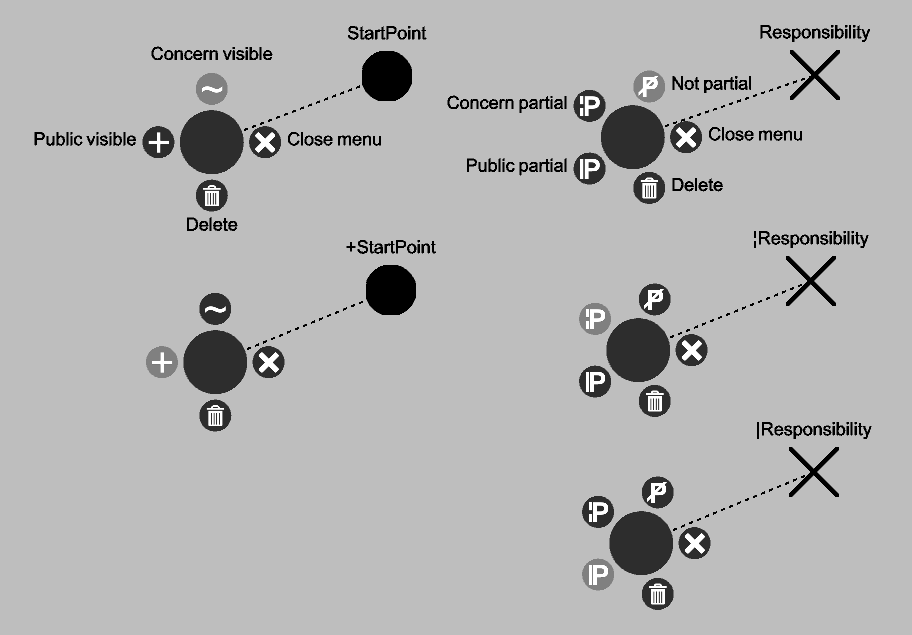
\includegraphics[scale=0.3]{fig_4_3.png}
	\caption{Visibility and partiality}
	\label{fig:4.3}
\end{figure}

Elements with extra features can be accessed by tap-and-hold an element (Figure~\ref{fig:4.3}). We allow start and end points to set its visibility. By default, all path nodes are concern visible, but start and end points can switch to public visible (see Section~\ref{sec:3.2.1.1} for visibility discussion). Likewise, we allow responsibilities to set its partiality. By default, all path nodes are not partial, meaning they are well-defined and require no further action. Since we have customization mappings for responsibility, we can specify whether a responsibility is partially defined and require appropriate composition to be semantically complete. A responsibility that is concern partial should fulfill its significance through model extension, whereas a responsibility that is public partial should fulfill its significance through model reuse.

\subsection{Scenario Model Composition}

\subsubsection{Model Extension}

\begin{figure}
	\centering
	\subfloat[Model A - parent UCM]{\label{fig:4.4a}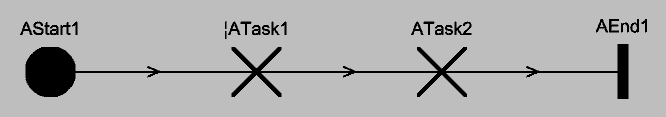
\includegraphics[clip,width=0.7\columnwidth]{fig_4_4a.png}} \\
	\subfloat[Model B - child UCM]{\label{fig:4.4b}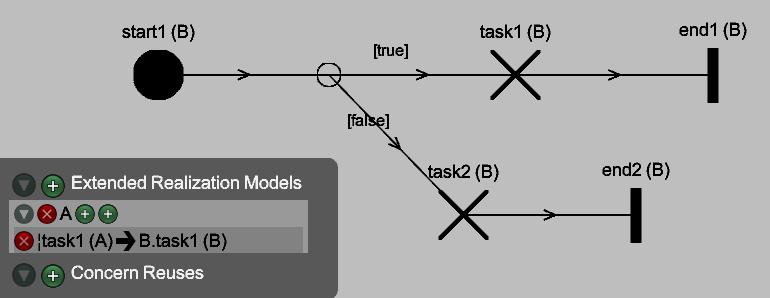
\includegraphics[clip,width=0.7\columnwidth]{fig_4_4b.png}} \\
	\subfloat[Woven Model B\_A]{\label{fig:4.4c}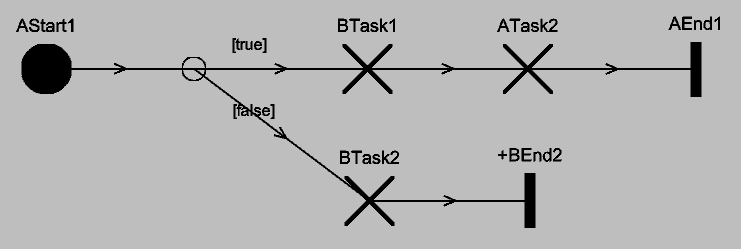
\includegraphics[clip,width=0.7\columnwidth]{fig_4_4c.png}}
	\caption{Schematic representation of model extension}
	\label{fig:4.4}
\end{figure}

Figure~\ref{fig:4.4} illustrates the usage of UCM model extension within a concern. Given a concern with two features in a hierarchy, the model of a child feature (Model B) extends the model of a parent feature (Model A). Composition specifications are specified in Model B, where an element of Model A is mapped to an element of Model B. Multiple mappings can be set per extension as needed and the available types of mapping are defined in the metamodel. The result of weaving Model B to Model A is depicted in Figure~\ref{fig:4.4c}. Based on the mappings set in Model B, the predecessors and successors of the mapped responsibility from Model B are introduced as adjoined path nodes of the mapped responsibility from Model A, and the mapped responsibility from Model A is being replaced with the mapped responsibility from Model B.

The idea of isolating features as individual models supports the use of advanced separation of concerns---each feature encapsulates its realization model. Features of a concern are nested in a hierarchical order, and the connection between features can be seen as parent-child relationship. Extension of a model depends on this relationship to ensure that models are woven in the correct order. Only the selected features of a concern are woven as a whole, providing only the absolute necessary details to fully describe the different use cases.

\subsubsection{Model Reuse}

\begin{figure}
	\centering
	\subfloat[Model C - reuse Concern A with selected features <A,B>]{\label{fig:4.5a}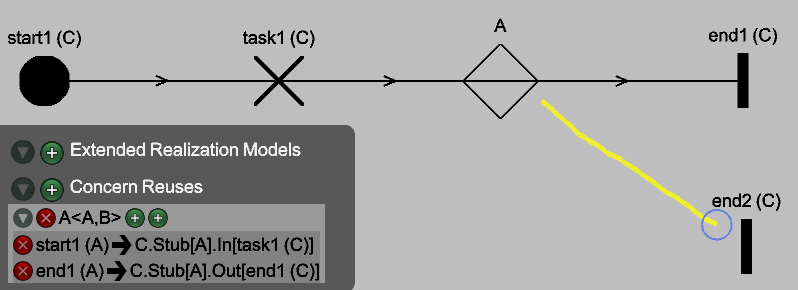
\includegraphics[clip,width=0.7\columnwidth]{fig_4_5a.png}} \\
	\subfloat[Model C - establish connecting point mapping through node connection]{\label{fig:4.5b}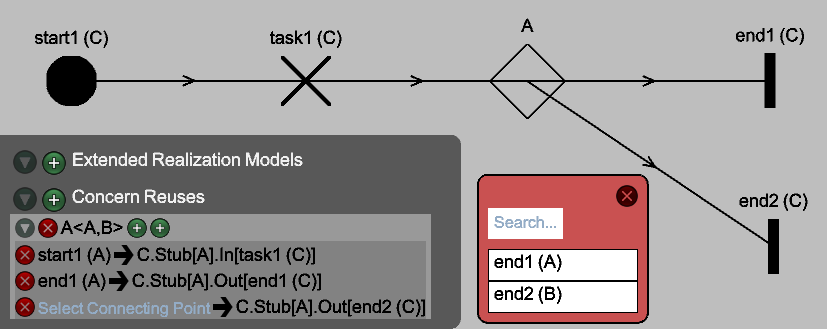
\includegraphics[clip,width=0.7\columnwidth]{fig_4_5b.png}} \\
	\subfloat[Woven Model C\_A<A,B>]{\label{fig:4.5c}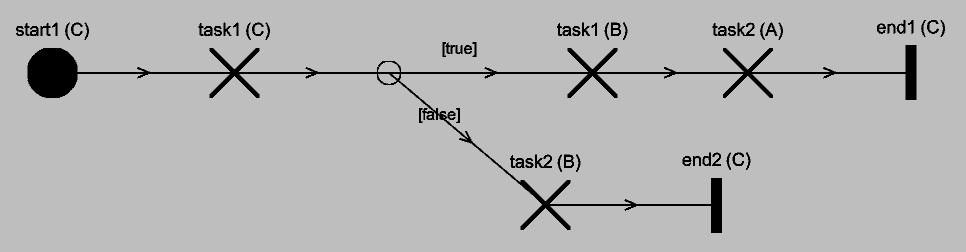
\includegraphics[clip,width=0.7\columnwidth]{fig_4_5c.png}}
	\caption{Schematic representation of model reuse}
	\label{fig:4.5}
\end{figure}

Figure~\ref{fig:4.5} illustrates the usage of UCM model reuse across concerns. Given that Model C of a concern reuses Concern A, the configuration for the set of features of Concern A will be displayed. Here, we chose to use features A and B, thus woven Model B\_A (see Figure~\ref{fig:4.4c}) is generated and represented as a static Stub A (appears automatically in canvas after successful reuse). Mappings for connecting points of Stub A can be established by linking a path node to/from Stub A. As shown in Figures~\ref{fig:4.5a} and~\ref{fig:4.5b}, a node connection was created from Stub A to an end point, and a list of end points from woven Model B\_A will be displayed for the user to set which end point of Model B\_A corresponds to which outgoing connection of Stub A in Model C. We label the incoming connection of a stub as \verb|<Model_2>.Stub[<Model_1>].In[<Predecessor>]|, and the outgoing connection as \verb|<Model_2>.Stub[<Model_1>].Out[<Successor>]|. The result of weaving Model C to Model B\_A is depicted in Figure~\ref{fig:4.5c}.

\section{Case Studies} \label{sec:4.2}

In this section, we attempt to validate our proposed technique for concern-oriented UCMs with two case studies: Authentication and Online Payment. We chose these two examples as our case studies because they provide different yet appropriate level of complexity to the problem that we are studying, as well as the ability to reuse the Authentication concern within the Online Payment concern.

\subsection{Authentication}

\begin{figure}[h]
	\centering
	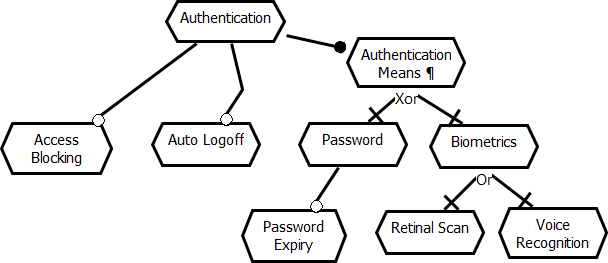
\includegraphics[scale=0.5]{fig_4_6.png}
	\caption[Feature model for Authentication (jUCMNav)]{Feature model for Authentication (jUCMNav). Image courtesy of Nishanth Thimmegowda et al.~\cite{thimmegowda2014concern}}
	\label{fig:4.6}
\end{figure}

We design the Authentication concern based on a reference model that we have previously described in jUCMNav format~\cite{thimmegowda2014concern}. Figure~\ref{fig:4.6} shows all the available features that are supported for the concern. \emph{Authentication} has a mandatory \emph{Authentication Means} feature that may either be \emph{Password} that can be extended with the optional \emph{Password Expiry} feature, or \emph{Biometrics} that requires at least \emph{Retinal Scan} or \emph{Voice Recognition}. If necessary, consecutive unsuccessful authentication attempts may result in \emph{Access Blocking} and long idle period may lead to \emph{Auto Logoff}.

\begin{figure}
	\centering
	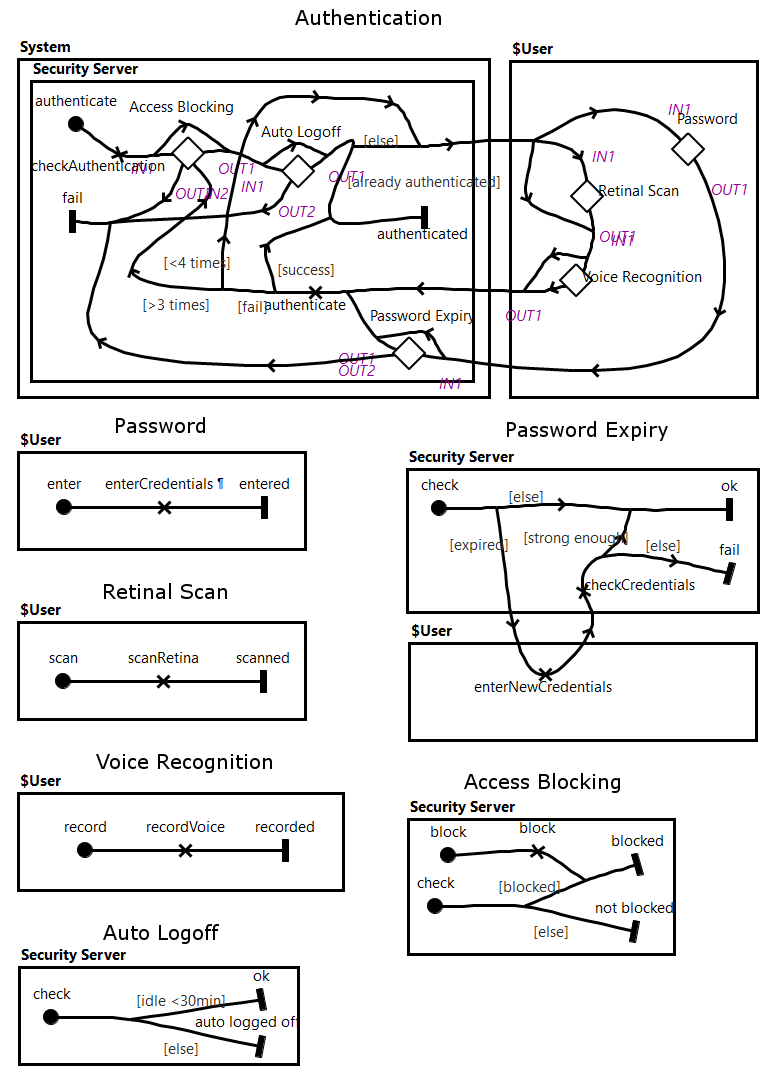
\includegraphics[scale=2]{fig_4_7.png}
	\caption[Scenario models for Authentication (jUCMNav)]{Scenario models for Authentication (jUCMNav). Image courtesy of Nishanth Thimmegowda et al.~\cite{thimmegowda2014concern}}
	\label{fig:4.7}
\end{figure}

\begin{figure}
	\centering
	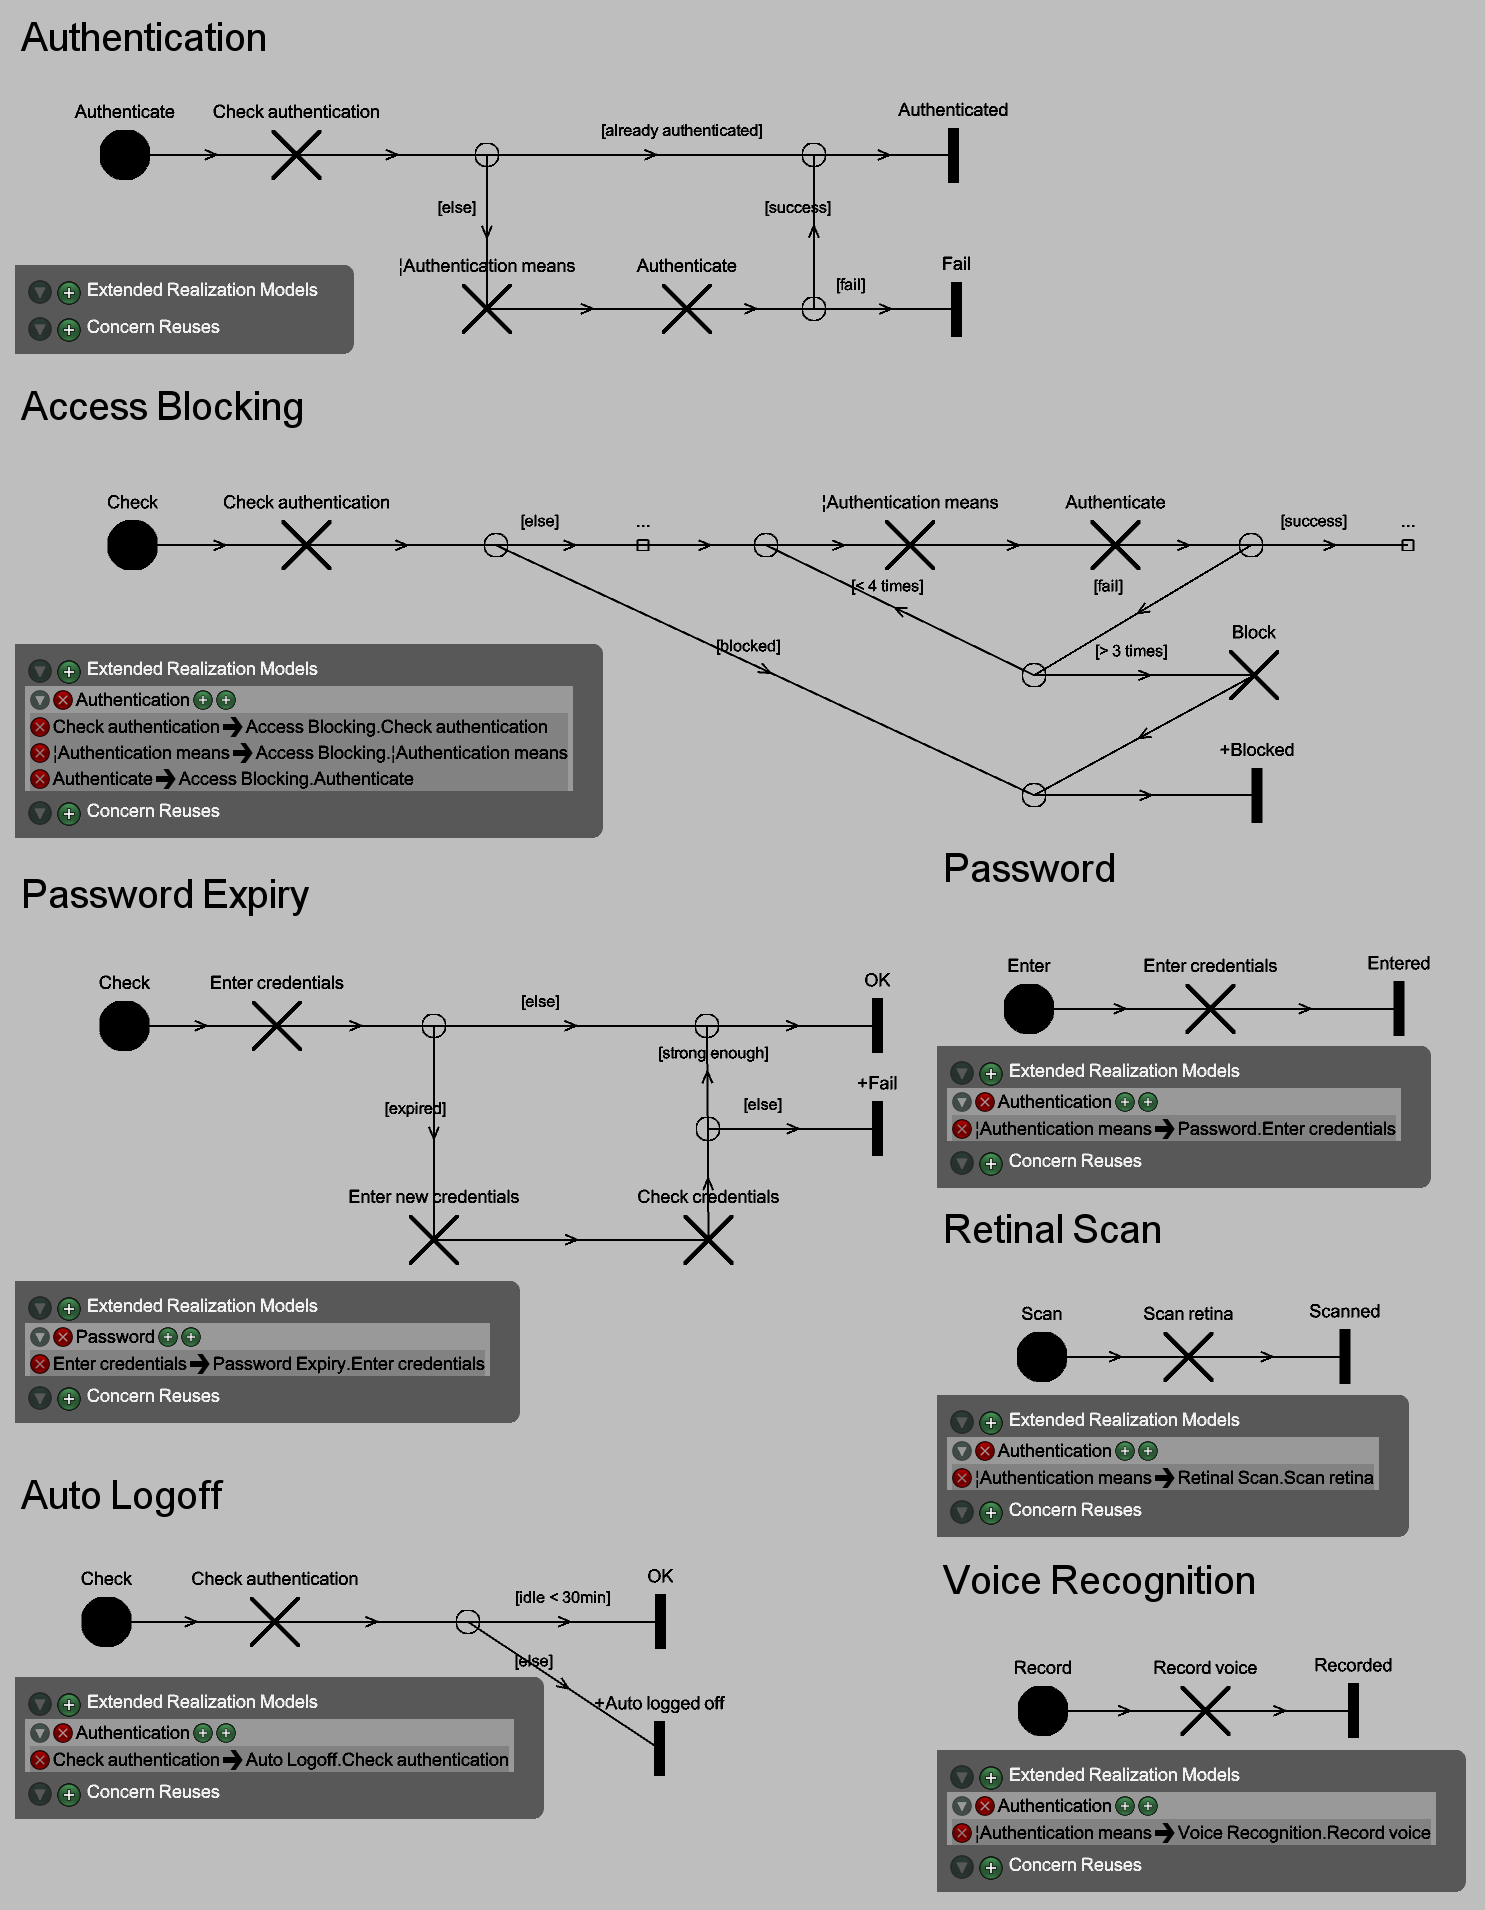
\includegraphics[scale=1.2]{fig_4_8.png}
	\caption{Scenario models for Authentication (TouchCORE)}
	\label{fig:4.8}
\end{figure}

Scenario models can be (optionally) realized for the features to describe how the user would interact with the Authentication concern. Figure~\ref{fig:4.7} illustrates the UCM diagrams and plug-ins that are realized for most of the features. Then, with slight modifications to the UCMs specified in jUCMNav, we developed our version of the UCMs using TouchCORE as depicted in Figure~\ref{fig:4.8}. (Feature model remains unchanged and TouchCORE version of the feature model is omitted.)

Notice that in the root map of Figure~\ref{fig:4.7}, each feature is represented as a static stub and is bound to a plug-in for the feature. In the root map developed using TouchCORE (see Figure~\ref{fig:4.8}), we minimize the usage of stubs and instead utilize model extensions, successfully isolating the aspects of crosscutting the core concern. Since \emph{Authentication Means} is a mandatory feature, we introduce a responsibility placeholder and set its partiality to concern partial. Any UCMs under the \emph{Authentication Means} feature can extend the root UCM via responsibility mapping. One advantage of using CORE approach in modeling UCMs is that by selecting the desired features when reusing this concern, only the UCMs of those selected features will be composed into the root map and a single UCM that consists of only the necessary paths will be generated. The woven UCM can be reused in another concern such as Online Payment.

\subsection{Online Payment}

\begin{figure}[h]
	\centering
	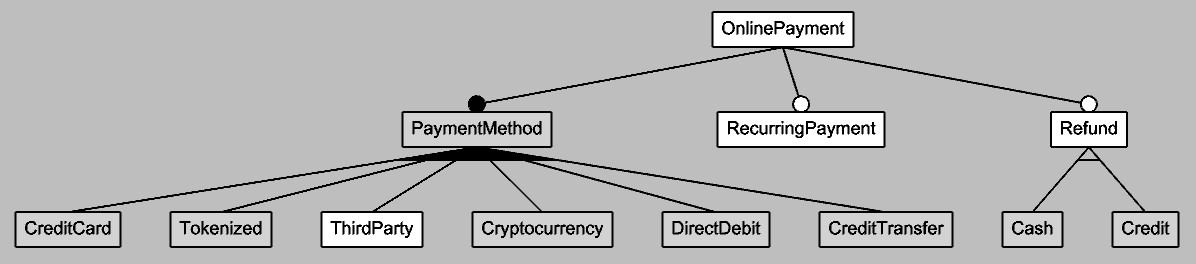
\includegraphics[scale=1.5]{fig_4_9.png}
	\caption{Feature model for Online Payment}
	\label{fig:4.9}
\end{figure}

\begin{figure}
	\centering
	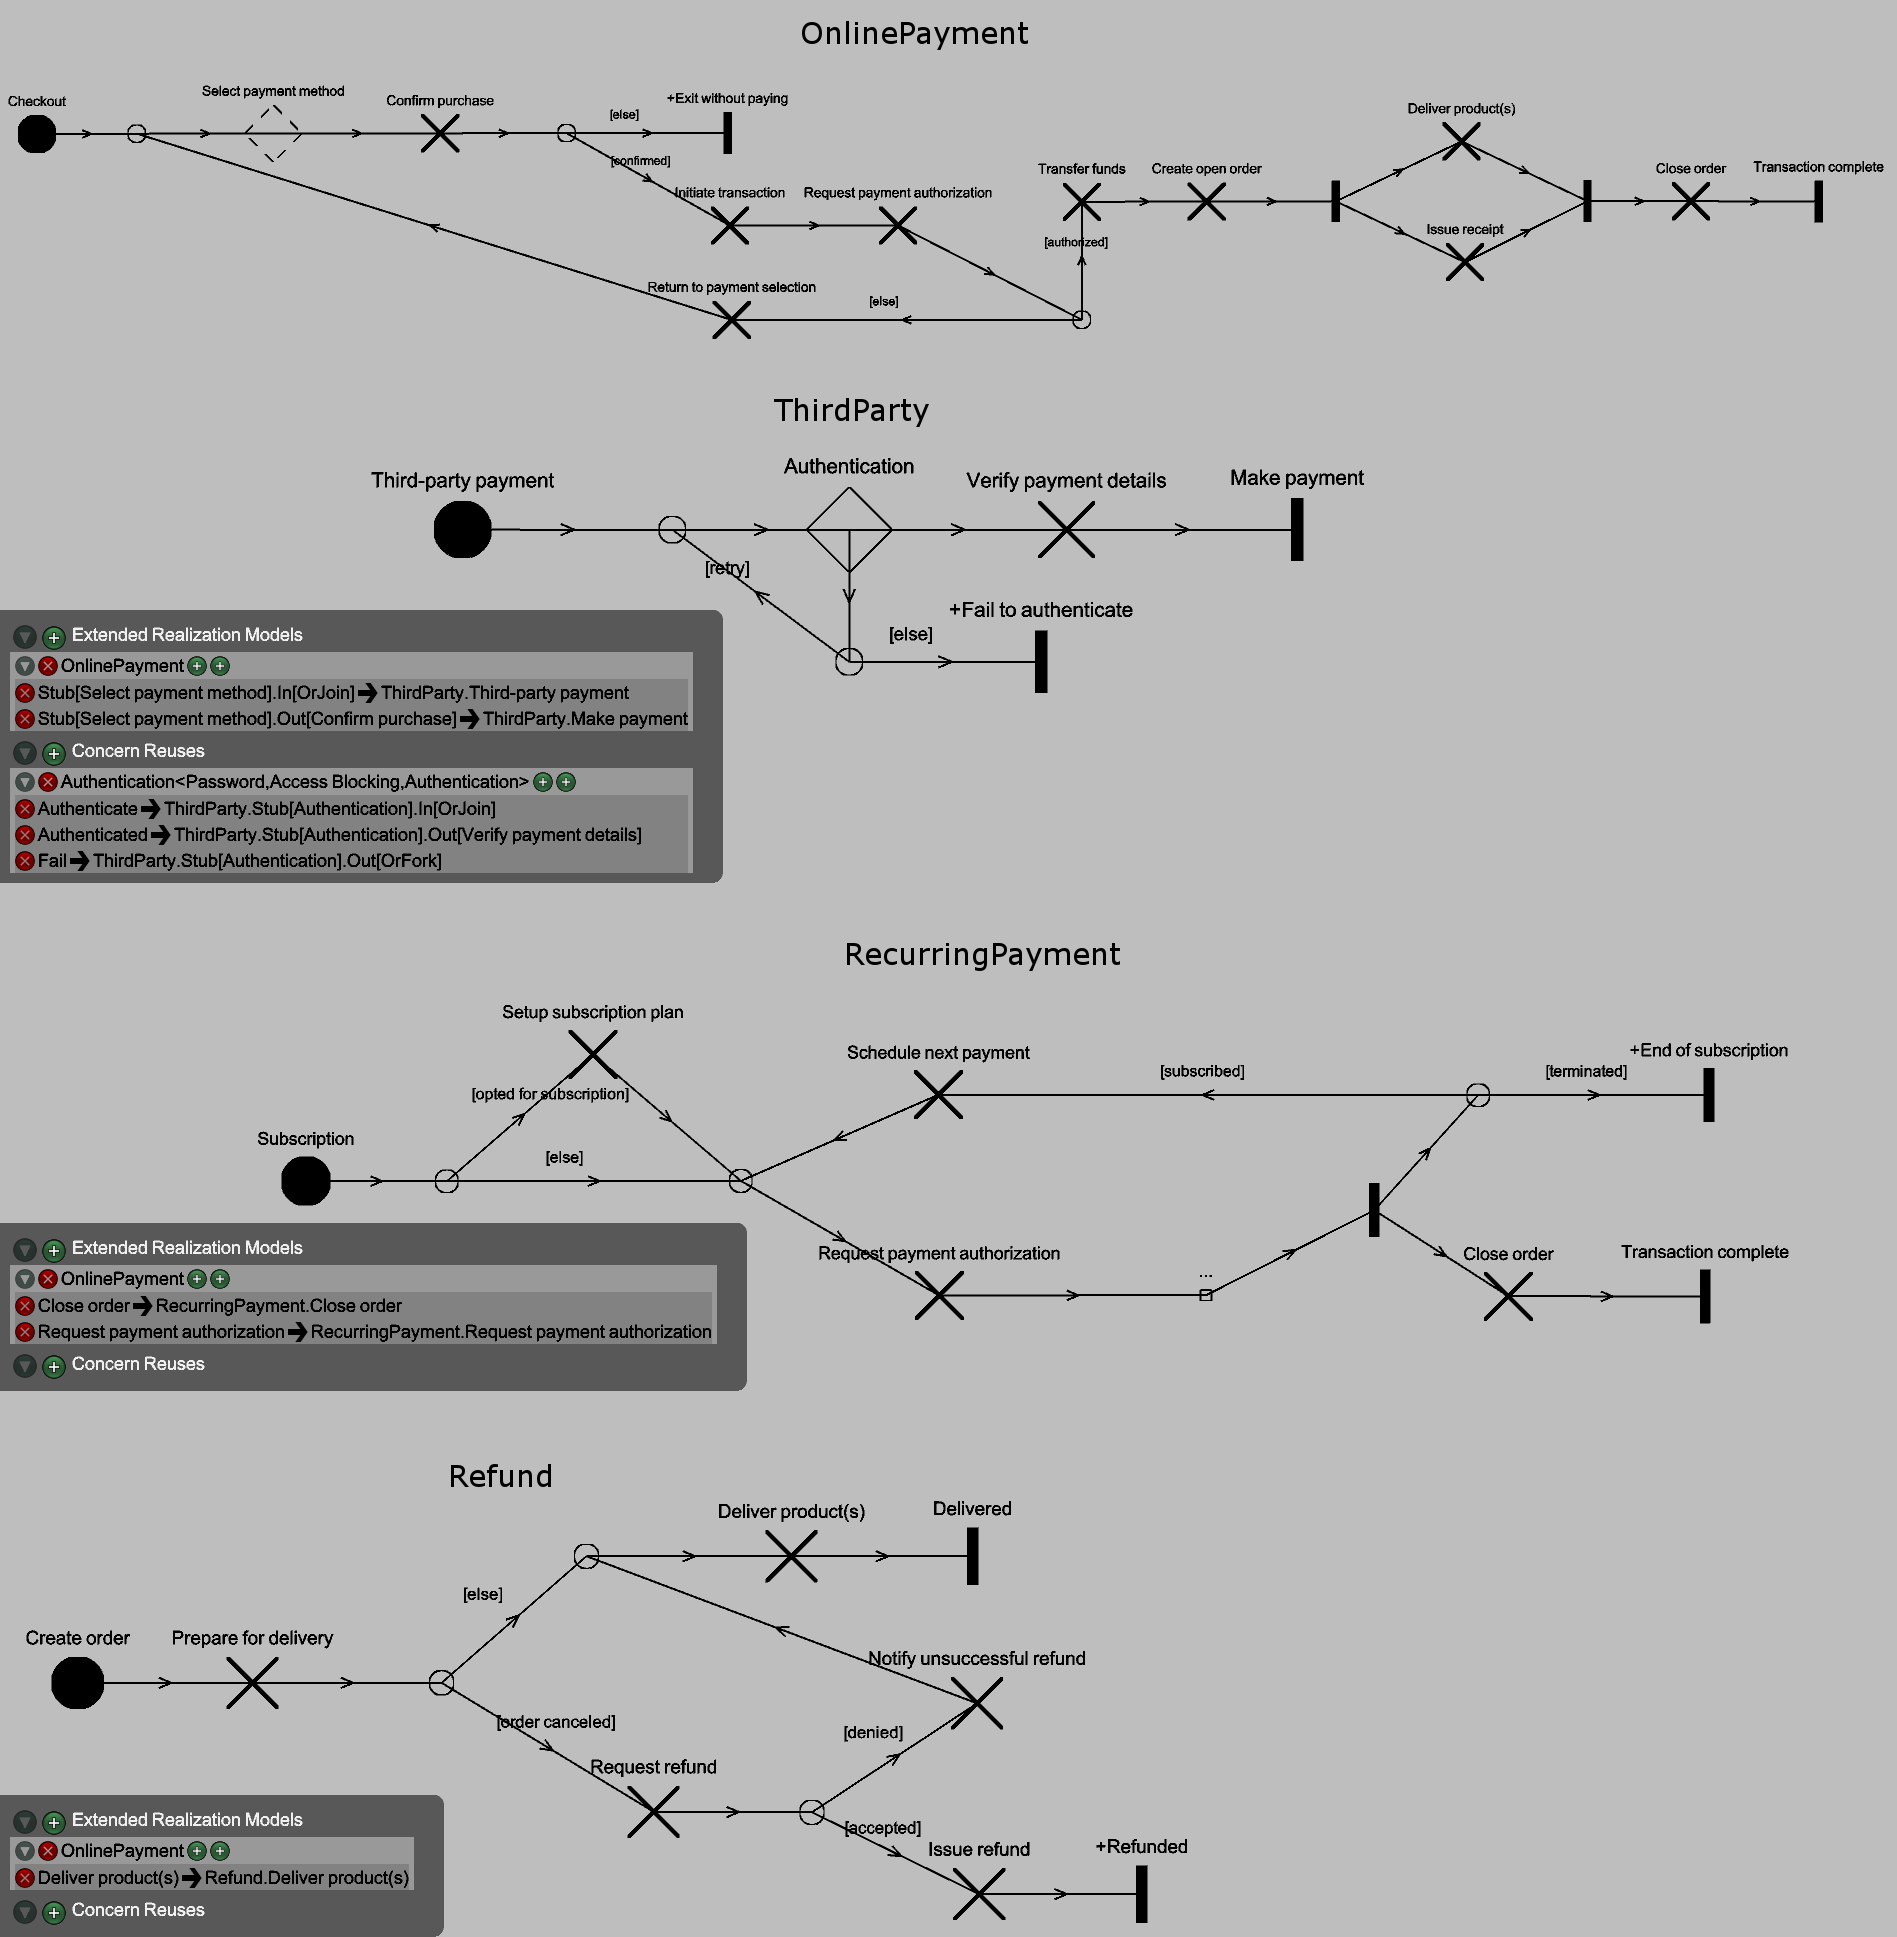
\includegraphics[scale=1]{fig_4_10.png}
	\caption{Scenario models for Online Payment}
	\label{fig:4.10}
\end{figure}

The Online Payment concern offers a means to build a payment model for e-commerce platform. Use cases for Online Payment are adapted from W3C Web Payments Interest Group \cite{w3c2015web}, focusing on the payment schemes in use today. Figure~\ref{fig:4.9} shows all the available features that are supported for the concern. Online Payment provides numerous payment methods for the customers to pay by credit card (e.g., Visa, MasterCard, China UnionPay), tokenized payment (e.g., ApplePay, Venmo, CyberSource), third-party payment (e.g., PayPal, Alipay, Google Pay), cryptocurrency (e.g., Bitcoin, Ripple, Ethereum), direct debit, or credit transfer. Optionally, the system supports recurring payment option to allow for subscription plan and refund to the payer's payment instrument or store credit.

Figure~\ref{fig:4.10} illustrates a typical workflow for Online Payment. In the root map, we have a single entry and exit point---from checkout to transaction complete---and a loop that redirects the user back to the payment selection if payment authorization fails. The payment method selection is modeled as a dynamic stub to receive multiple plug-ins from the subfeatures of \emph{PaymentMethod}. We limit the discussion of \emph{PaymentMethod} to \emph{ThirdParty} since the scenario model for paying through third-party is sufficient to describe the essential features and most methods share similar scenario. There are two things worth mentioning in the \emph{ThirdParty} model. First, \emph{ThirdParty} extends \emph{OnlinePayment} through the \emph{Select payment method} dynamic stub, hence mapping is done via connecting points. Second, \emph{ThirdParty} reuses the Authentication concern is depicted as a static stub, and the selected features are \emph{Password} and \emph{Access Blocking}. The one incoming connection and two outgoing connections of the \emph{Authentication} stub are associated with the single start point (\emph{Authenticate}) and two end points (\emph{Authenticated}; \emph{Fail}) of Authentication UCM (see Figure~\ref{fig:4.8}).

Optional features of \emph{OnlinePayment} are \emph{RecurringPayment} and \emph{Refund}. Both of the features extend \emph{OnlinePayment}. For \emph{RecurringPayment}, the {\cls Anything} node represents the sequence of nodes on the path of \emph{OnlinePayment}---from \emph{Request payment authorization} to \emph{Close order}---and a loop to enable recurring payment is injected in between the two responsibilities. The \emph{Refund} model we defined here is restricted to the refund policy that allows customers to request for refund after they made the payment, but prior to receiving the goods. Refund after the delivery of product(s) requires a separate UCM and is outside the scope of this case study.

The purpose of these case studies is to demonstrate the application of model reuses, such as the reuse of Authentication concern in the \emph{ThirdParty} UCM model, as well as model extensions via responsibility mappings and connecting point mappings. Successful application of extensions and reuses allows for the development of scalable and reusable scenario models through TouchCORE. Concerns can be as fine-grained as Authentication, or intermediate concerns that reuses Authentication such as Online Payment, up to a proper application (e.g., electronic commerce websites) that reuses Online Payment.

\section{Workflow Patterns} \label{sec:4.3}

This last section demonstrates the use of concern-oriented UCMs to implement some of the workflow patterns described by van der Aalst et al.~\cite{van2003workflow}. We chose to cover two of the state-based patterns---\emph{Deferred Choice} and \emph{Milestone}---as they present the appropriate level of complexity, given that some of the workflow patterns are primitive and already supported by the standard UCM notations, as well as the constraints imposed by our partial implementation of UCM notations in TouchCORE.

\subsection{Deferred Choice}

The deferred choice pattern allows the moment of choice to be suspended as late as necessary---process can only continue based on external factors. In essence, all branches represent possible future courses of execution. Only once the decision has been made to proceed with a particular branch, execution for the other branches come to a halt. 

\begin{figure}[h]
	\centering
	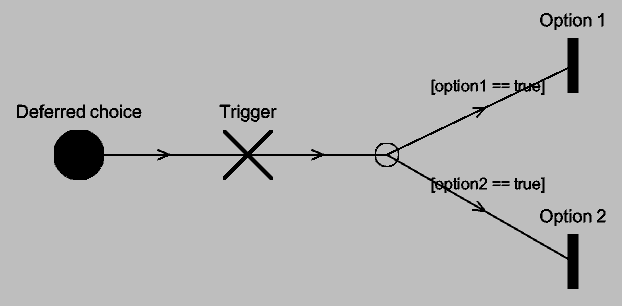
\includegraphics[scale=1.3]{fig_4_11.png}
	\caption{Deferred choice pattern}
	\label{fig:4.11}
\end{figure}

Typical implementation of deferred choice is using an AND-fork to enable all parallel branches. After one of the branches has started processing, all other branches are canceled. Since the UCM notation does not have the ability to signal for cancellation of other branches, an alternative strategy is the use of XOR-split. Figure~\ref{fig:4.11} illustrates the OR-fork implementation for the deferred choice pattern; the \emph{Trigger} is responsible for activating the proper branch, by setting $option_1$ to $true$ and $option_2$ to $false$ or vice versa. The pattern is realized as a feature in a concern and can be reused in other UCMs. One example of reuse is in the milestone pattern.

\subsection{Milestone}

The milestone pattern supports the conditional execution of a task only if a parallel process is in a given state, i.e. an activity can only be enabled if a certain milestone has been reached and has not expired yet. Different strategies exist for the implementation of the milestone pattern, and one form uses a deferred choice in the workflow. Deferred choice offers two subsequent activities and is modeled with an OR-fork within the reused Deferred Choice concern. The path to one activity is enabled only after reaching a milestone, after which the path merges prior to the deferred choice construct and the same activity can be executed repeatedly, given that the current state is still in the milestone. On the other hand, if the current state leaves the milestone, then the path to the first activity is disabled by the OR-fork, leaving only the path to the second activity.

\begin{figure}
	\centering
	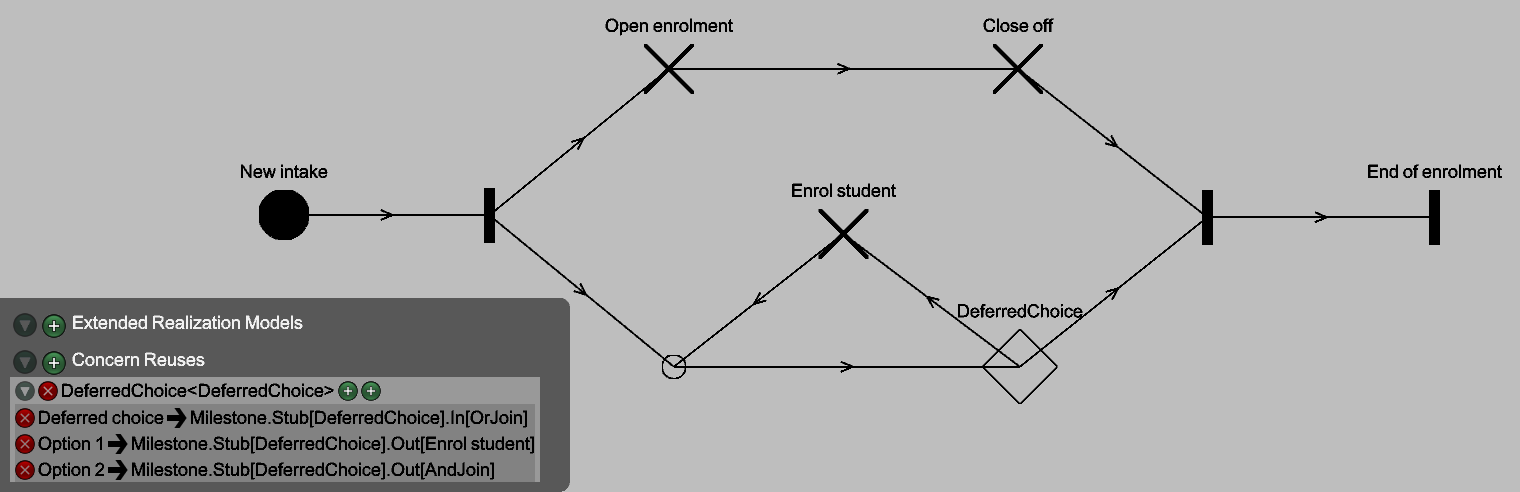
\includegraphics[scale=1.3]{fig_4_12.png}
	\caption{Milestone pattern (enrolment example)}
	\label{fig:4.12}
\end{figure}

Whereas the deferred choice pattern is modeled as a reusable concern, the milestone pattern is implemented slightly different. We took an example of student enrolment, applying the milestone pattern (deferred choice implementation), as shown in Figure~\ref{fig:4.12}. New enrolments are being accepted when the enrolment period opens (at the point of reaching a milestone) until the enrolment period closes (at the point of deadline) for a given intake. Ideally, the route to \emph{Enrol student} ($option_1$) can only be activated when the token on the other parallel path reaches \emph{Open enrolment} but before reaching \emph{Close off}. All other instances would result in inaccessible path $option_1$, leading to the only exit path available that is \emph{End of enrolment} ($option_2$).


\chapter{Conclusion} \label{ch:5}
\section{Summary}

Requirements elicitation forms a fundamental piece of software engineering and is typically performed at the initial phase of the software development process. This thesis introduces CoUCM that consolidates scenario modeling with advanced SoC, MDE, and SPL. Along with the already existing GRL support for goal modeling in CORE, the addition of UCM offers a complete URN package for requirements engineering in CORE.

The proof of concept implementation of CoUCM in TouchCORE demonstrates the project's feasibility. TouchCORE is a modeling tool that provides an intuitive interface for concern-oriented software design. Both CoUCM and RAM allow TouchCORE users to model at different level of abstractions, covering the requirements and design phases. In addition, modelers can now populate the TouchCORE library with reusable scenario models encoding essential recurring requirements concerns (e.g., functional units, workflow patterns, etc).

Limitations of the work exists, however, and serve as potential future work for improvements, which we discuss in the next section.

\section{Future Work}

The integration of UCM to CORE has not been completed yet, specifically the use of {\cls ResponsibilityRef}s to refer to a particular {\cls Responsibility} definition from multiple reference points that belong to other UCMs, as well as the use of {\cls Component}s to model the architectural structure of a system. Implementation of {\cls Component} to CoUCM poses some difficulties especially when taking model composition into account as responsibilities within a component are bound to the component. Several other model elements including waiting place, timer, failure point, and abort could be added to the CoUCM metamodel to complete the standard UCM features.

Similarly, the implementation of scenario modeling to TouchCORE is in the alpha phase. TouchCORE features such as traceability and model validation could be implemented to allow for a better scenario modeling experience. Path drawing could be improved as current implementation uses straight lines to connect path nodes; splines would work well if supported by TouchCORE GUI. One of the jUCMNav tool's features is the path traversal mechanism~\cite{kealey2007enhanced2}. If implemented in TouchCORE, this mechanism allows for UCM analysis and is particularly useful in evaluating scenario variables when traversing paths.

Supplementary work to the CORE base design is needed to allow a more seamless integration of multiple modeling languages. Since this is one of the early works (after RAM) that extends a modeling language (UCM) with concern-orientation, future addition of modeling languages to CORE can refer to this work as reference. We hope that this work would motivate future studies to further improve the CORE paradigm.


%----------------
% End Matter
%----------------
\begin{appendices}

\chapter{Complete Metamodels}
\section{CORE Metamodel}

\begin{figure}[h]
	\centering
	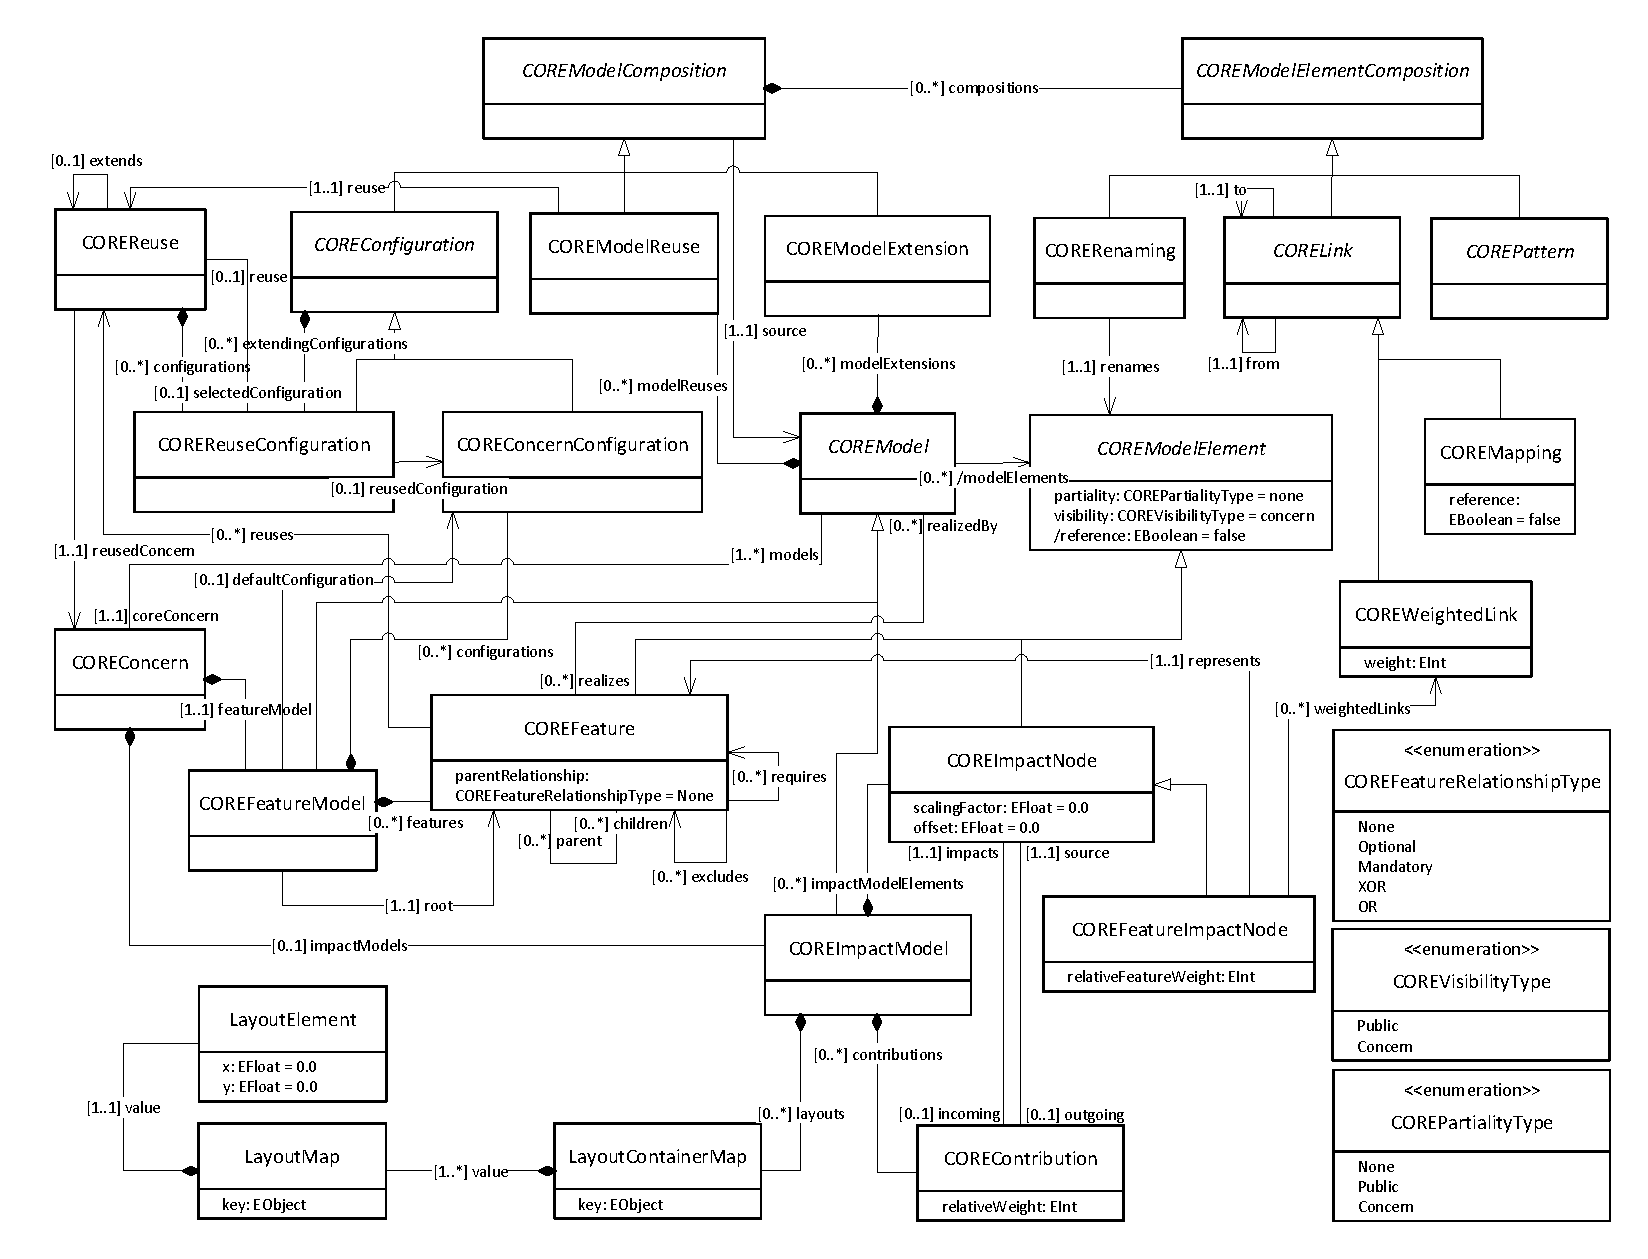
\includegraphics[scale=0.59]{fig_a_1.pdf}
	\caption{Abstract grammar: CORE metamodel overview}
	\label{fig:a.1}
\end{figure}

\section{UCM Metamodel}

\begin{figure}[h]
	\centering
	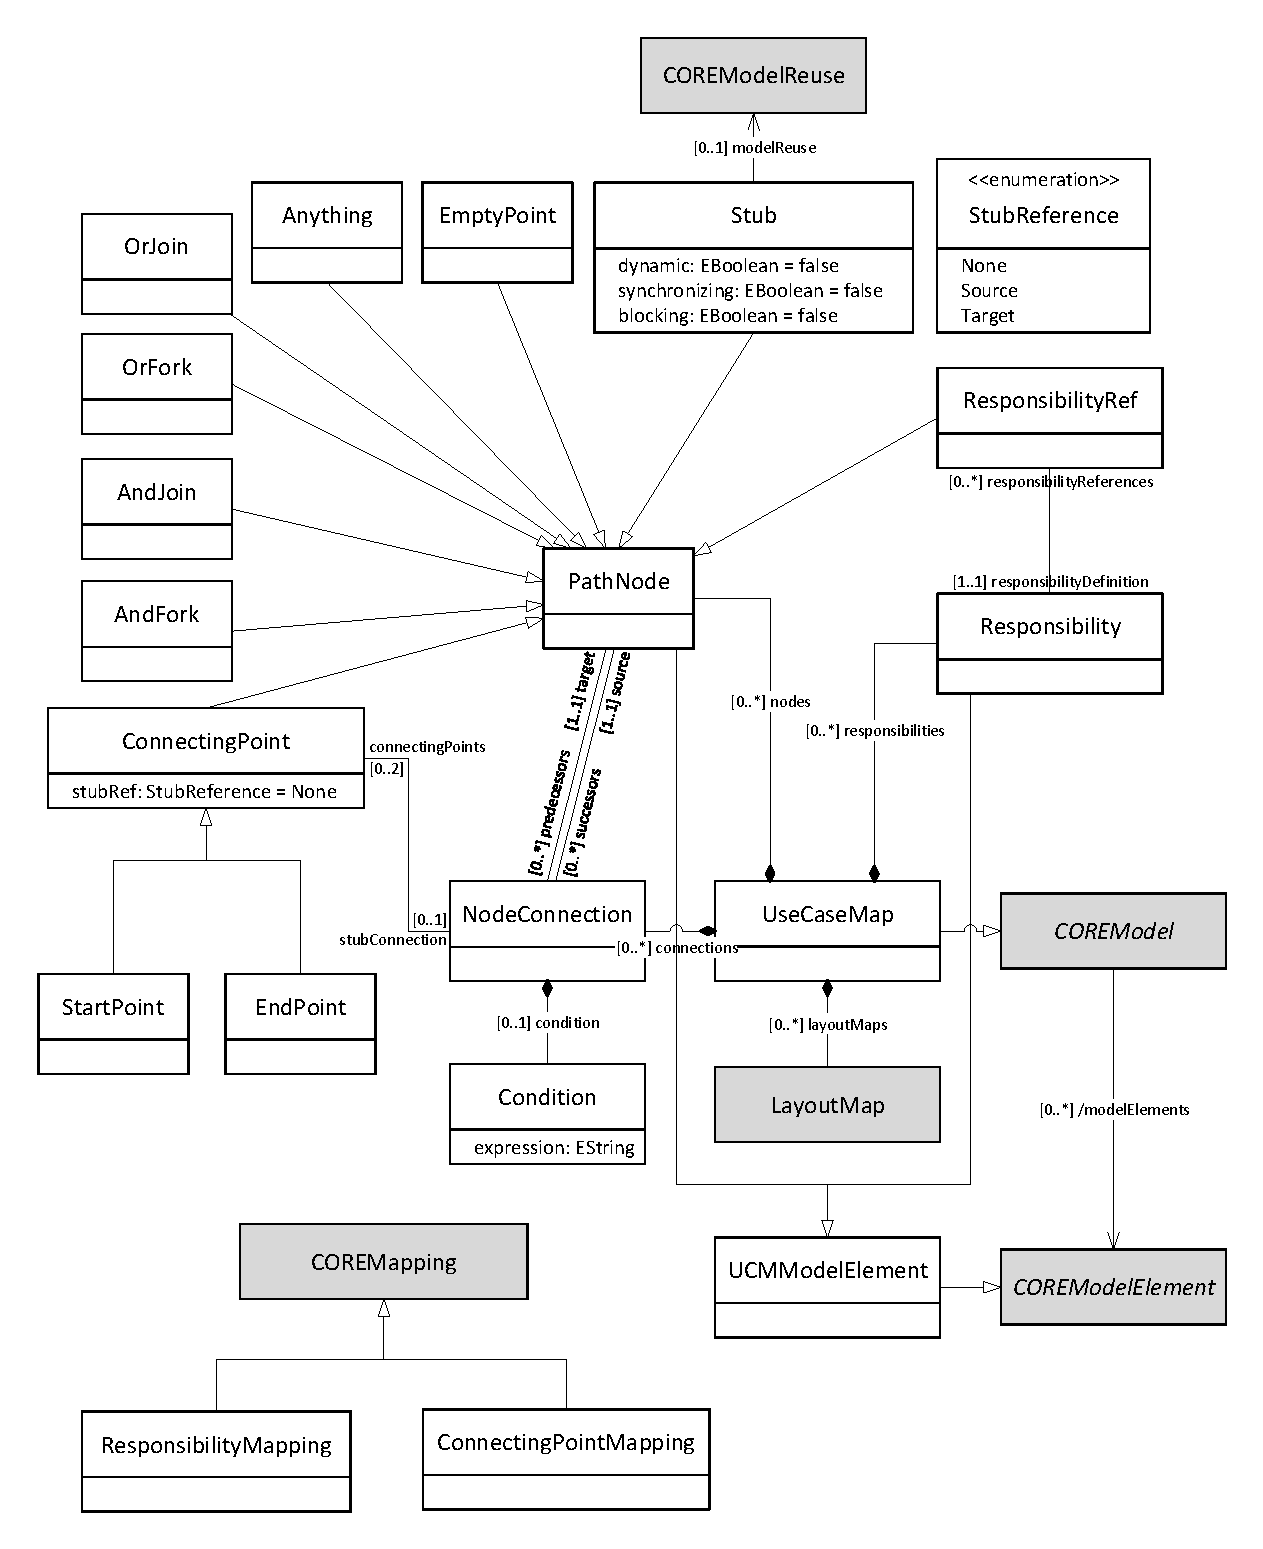
\includegraphics[scale=0.53]{fig_a_2.pdf}
	\caption{Abstract grammar: UCM metamodel overview}
	\label{fig:a.2}
\end{figure}


\chapter{Complete Case Study Models}
\section{Authentication Model}

\section{Online Payment Model}


\end{appendices}

\renewcommand\bibname{References}
\printbibliography[heading=bibintoc]

\end{document}
